\documentclass[conference,9pt]{IEEEtran}
\usepackage{xcolor}
\usepackage{cite}
\usepackage{epsfig}
\usepackage{amssymb}
\usepackage{amsmath}
\usepackage{graphicx}
\graphicspath{ {./} }

\begin{document}
\title{Practical 3a}

\author{
\IEEEauthorblockN{Albert Acebron}
\IEEEauthorblockA{NIU: 1458626}
}


% make the title area
\maketitle
\begin{abstract}
This practical will be based on estimating the frequency of two signals that have been combined into one.
\end{abstract}

\section{Questions}

\subsection{Question 1}
Using the (2.4) formula:
\begin{verbatim}
  function S_per = compute_periodogram(signal)
    n=length(signal);
    S_per=abs(fft(signal)).^2/n;
  end
\end{verbatim}


\subsection{Question 2}

Given that the sampling frequency is 10MHz, a segment of length $m \mu s$ will be contained in $10^{6-6+1}*m$ discrete samples, which means that, to analyze segments of lengths $10\mu s, 100\mu s, 500\mu s$, we will use 100, 1000 and 5000 samples respectively.

Next we will take these segments and calculate their periodogram, get their maximums and convert these to frequency values\footnote{Due to the fact that the periodogram covers the frequencies from 10MHz/N to 10MHz (the sampling freq), the bins will have a size of $\frac{10MHz}{N}$ where N is the number of samples used} with the following code:
\begin{verbatim}
  for k=[100, 1000, 5000]
    Px=perio(RxSignal(1:k));
    peaks = peakDetector(Px, 2)*10^7/k
  end
\end{verbatim}

The resulting estimated frequencies are:
\begin{center}
  \begin{tabular}{ c c c c c c c c c c }
    Length & First freq & Second freq \\
    $10\mu s$ & 1.2MHz & 1.1MHz \\
    $100\mu s$ & 1.13MHz & 1.07MHz \\
    $500\mu s$ & 1.126MHz & 1.058MHz \\ 
  \end{tabular}
\end{center}

As we can appreciate, an increase of the number of samples used gets us higher precision in our results.

\subsection{Question 3}
To calculate the periodogram we are using a same-size DFT, and this means that the resulting vector will be on the frequency range from Fs/N to the sampling frequency (10MHz in this case), with a number of bins equal to the number of samples that were used to create the periodogram.

This means that the resolution of our result will be $\frac{10MHz}{N}$, but if we were to normalize the frequencies (so they go from 0 to 1 instead) this would become $\frac{1}{N}$. With this equation we can obtain the number of samples needed to achieve a resolution of 0.0002 by simply solving the following equation.
$$\frac{1}{N}=0.0002$$

Which yields the result:
$$N=\frac{1}{0.0002}=5000$$

\subsection{Question 4}
\begin{verbatim}
  N=5000;
  Px=perio(RxSignal(1:N));
  Px=Px.*(max(abs(RxSignal(1:N)))/max(Px));
  x=Fs/N:Fs/N:Fs;
  plot(x, Px)
\end{verbatim}

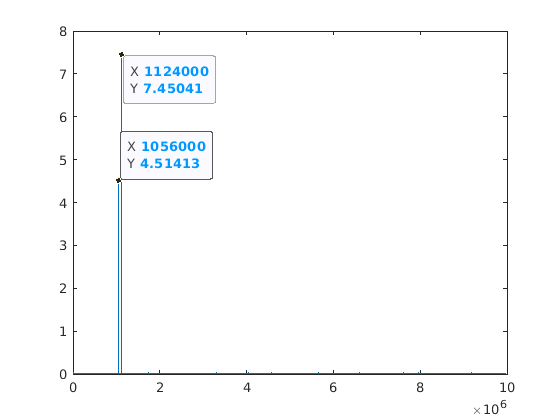
\includegraphics[scale=0.6]{q4}

As shown on the figure, the estimated frequencies are 1.056MHz and 1.124MHz.

\subsection{Question 5}
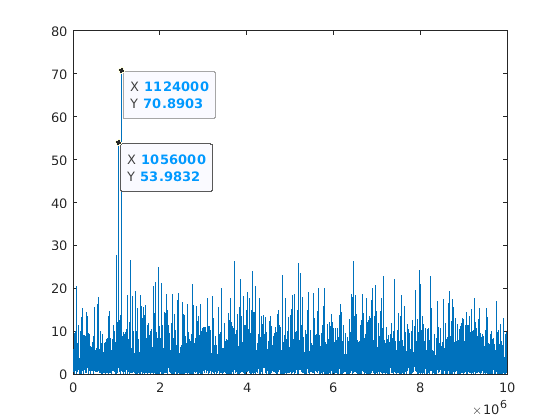
\includegraphics[scale=0.6]{q5}

In the spectrum of this signal we see much more noise across the spectrum but we can still make out two peaks at 1.056MHz and 1.124MHz, which are the frequencies we are looking for.

We can't tell which of these is the frequency of interest as we don't have enough data.

\subsection{Question 6}
We'll begin by estimating the biased autocorrelation using the xcorr function from Matlab (xcorr's also provides the negative values of the correlation so to get the it to start at x=0 we'll remove the first half of the results):
\begin{verbatim}
  rx=xcorr(signal, 'biased');
  rx=rx(N:end);
\end{verbatim}

Then let's construct the matrixes:
\begin{verbatim}
  r=rx(2:p+1);
  R=toeplitz(rx(1:p), conj(rx(1:p)));
\end{verbatim}

Solve for $a$ and $\sigma_w$:
\begin{verbatim}
  ar=-inv(R)*r;
  a=[1; ar];
  sigma=rx(1)+ar'*r
\end{verbatim}

The resulting sigma is $2.0108e+04 + 2.2737e-13i$, which should be a real number, but as we can see, it's a complex one. However, the complex part of the number is extremely insignificant compared to the real one (concretely, there's 17 magnitudes of difference between them) so we'll assume it's a numerical calculation error and eliminate it:
\begin{verbatim}
  sigma=real(sigma); % Remove numerical error
\end{verbatim}

And construct the final result:
\begin{verbatim}
  Sx=sigma./(abs(fft(a)).^2)
\end{verbatim}

We could just leave it like this, but, for convenience, to get the same number of points that the periodogram from before has, which will make comparisons easier, we'll compute the fft with N points:
\begin{verbatim}
  Sx=sigma./(abs(fft(a, N)).^2)
\end{verbatim}

Putting it all together:
\begin{verbatim}
function S_AR = compute_AR(signal, p)
  N=length(signal);
  rx=xcorr(signal, 'biased');
  rx=rx(N:end);
  r=rx(2:p+1);
  R=toeplitz(rx(1:p), conj(rx(1:p)));
  ar=-inv(R)*r;
  a=[1; ar];
  sigma=rx(1)+ar'*r;
  sigma=real(sigma); % Remove numerical error
  S_AR=sigma./(abs(fft(a, N)).^2);
end
\end{verbatim}

\subsection{Question 7}
We'll reuse the code from question 4:
\begin{verbatim}
  for p=[10, 100, 1000]
    N=5000;
    Px=compute_AR(RxSignal(1:N), p);
    Px=Px.*(max(abs(RxSignal(1:N)))/max(Px));
    x=Fs/N:Fs/N:Fs;
    plot(x, Px)
  end
\end{verbatim}

\pagebreak

Plot for $p=10$:

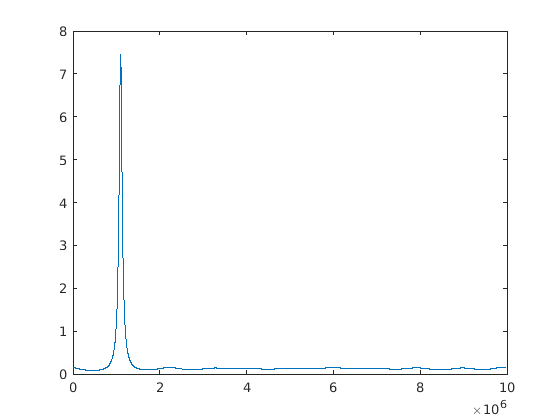
\includegraphics[scale=0.6]{p10}

Plot for $p=100$:

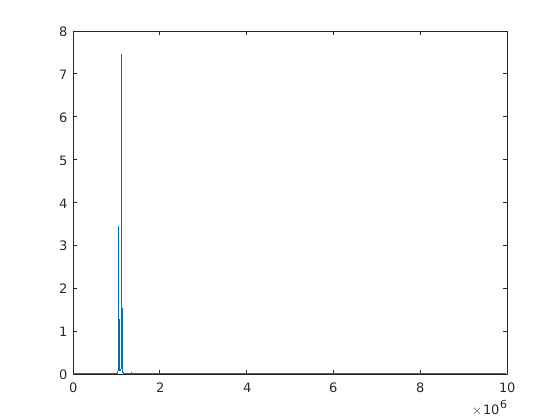
\includegraphics[scale=0.6]{p100}

Plot for $p=1000$:

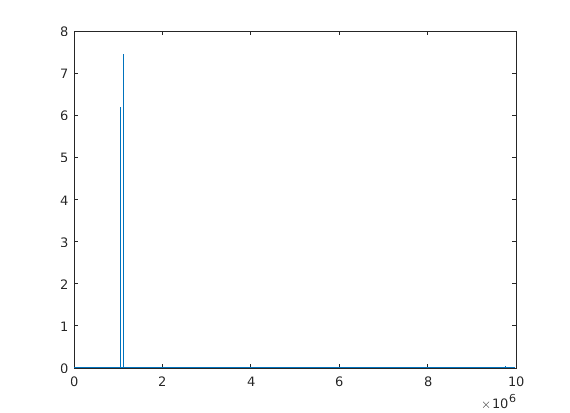
\includegraphics[scale=0.6]{p1000}

The plot where $p=1000$ is almost equal to the periodogram we computed earlier, whereas the one where $p=10$ resembles it a bit but is quite different and it's not possible to make out the two peaks, as they kind of get absorbed into a single peak. The plot made with $p=100$ is in the middle of these two: it's quite similar to the periodogram but not as much as the $p=1000$ plot.

In conclusion, the higher the value of $p$, the closer the plot resembles the one we got in the previous section.

\subsection{Question 8}

Using the code provided in question 7, we get the following plots with the noisy signal:

Plot for $p=10$:

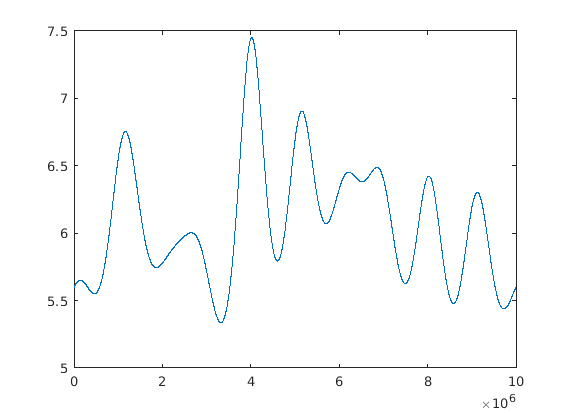
\includegraphics[scale=0.6]{pn10}

Plot for $p=100$:

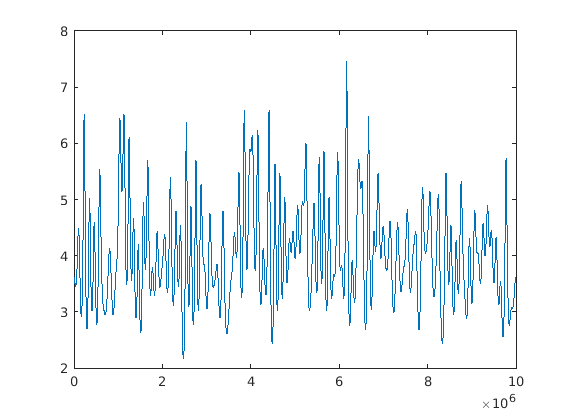
\includegraphics[scale=0.6]{pn100}

Plot for $p=1000$:

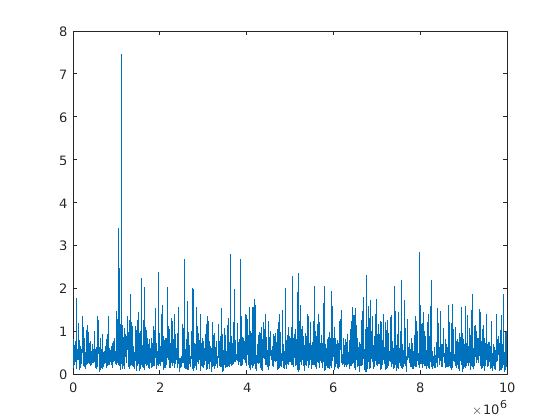
\includegraphics[scale=0.6]{pn1000}

In these graphs we can appreciate that graphs for $p=10$ and $p=100$ are completely different (this is because for low values of $p$ the autoregressive model used to estimate the signal isn't calculated properly when there's noise) whereas the graph for $p=1000$ matches the one we created in question 5.

Thus, to get a similar result the order of $p$ has to be close to $1000$.

\subsection{Question 9}

Advantages of using AR:
\begin{itemize}
  \item If $p$ is significatly smaller than the signal size, the computation required for the AR method\footnote{$O(p^2+n)$ due to the matrix multiplications being $O(p^2)$ and the correlation estimator adding $O(n)$} is smaller than the one required for the method used in the first section \footnote{$O(nlog(n))$ due to the fast fourier transform}.
  \item The plot of the AR spectogram for $p=1000$ and the noisy signal has a lower contribution from noise than the periodogram computed in question 5, so for noisy signals we might be able to get better results using the AR-based method.
\end{itemize}

Disadvantages:
\begin{itemize}
  \item If we pick a bad value for $p$ we might end up getting a wrong result
  \item If our signal cannot be properly modelled by the autoregressive model that AR uses (which assumes that any value of the signal can be estimated linearly from the previous $p$ values) then we are going to get wrong results
\end{itemize}

Due to the risks associated with having to pick a value for $p$ I'd recommend using the method based on the periodogram.

\end{document}


